\subsection{Data Collection}
	Data found through~\parencite{timeanddate.com} had to be processed before finding the averages of each month could be found.
Due to the data being represented as a series of string in columns in a text file, all values had to be converted into intergers.
This was due by usign python code to take the file, and separate each the string by the colon use in the values collected for times.


\subsection{Data Aanlysis}
	With sunrises times from all 365 days in 2024 available the averages of each month were taken.
This was done using the general formula for calculate mean.
$\text{Average} = \frac{Sum of times of each sunrise in the month}{Numer of days in the month}$

Once this was done for each month the twelve calculated averages were plotted on a graph with months over \ref{fig:sunrise}.

\begin{figure}[ht]
	\centering
	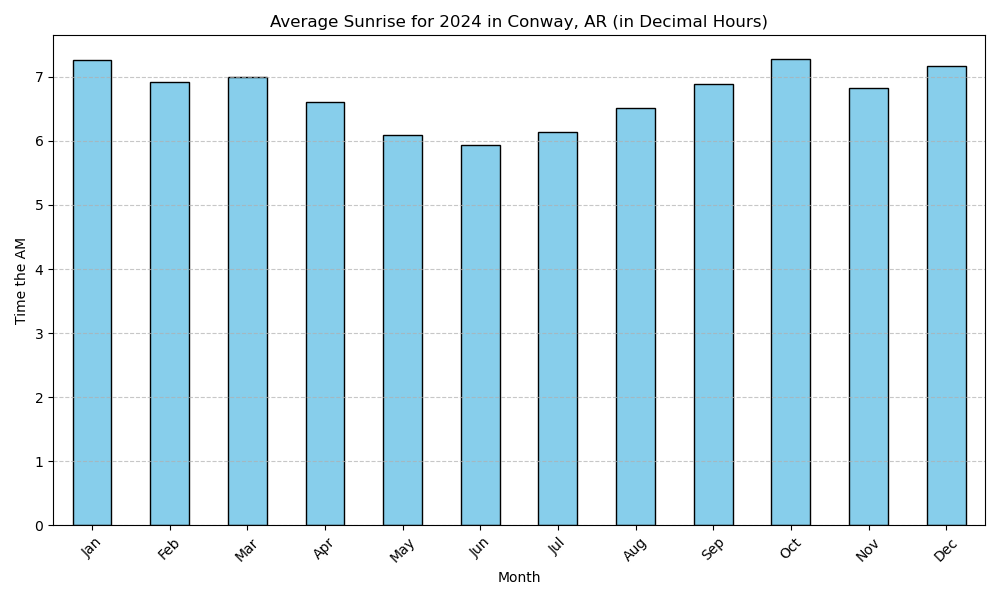
\includegraphics[width=0.7\textwidth]{Figure_1.png}
	\caption{Graph of the sunrise averages for each month in the year 2024}
	\label{fig:sunrise}
\end{figure}
